%%%%%%%%%%%%%%%%%%%%%%%%%%%%%%%%%%%%%%%%%%%%%%%%%%%%%%%%%%%%%%%%%%%%%%%%%%%%%%%%%%%%%%%%%
% Section 6: Placement in RapidSmith2
%	This section contains a description of the following:
%	- How to place cells onto BELs and map cell-pins to bel-pins in RapidSmith2
%	- How to get a list of valid placement locations for a cell  
%	- Placement special cases
%%%%%%%%%%%%%%%%%%%%%%%%%%%%%%%%%%%%%%%%%%%%%%%%%%%%%%%%%%%%%%%%%%%%%%%%%%%%%%%%%%%%%%%%%
\newpage
\section{Placement} \label{sec:placement}
\graphicspath{{./techReportFigures/sec6_placement/}}

In the original RapidSmith, placement occurred at the site level. A
collection of cells were grouped together into an \textit{instance}, and the
instance was assigned to a compatible site. The actual placement locations
for the cells within the site were unknown. Because RapidSmith2 breaks up a
site into its individual components, cells can now be placed directly onto
physical BELs within a site. This gives Xilinx FPGA CAD developers finer-grained
control over the placement of a design, and allows sub-site algorithms (such as
packers) to be explored. \autoref{code:place} demonstrates the basic steps to
placing cells in RapidSmith2.

\begin{lstlisting} [xleftmargin=1.5em, framexleftmargin=1.5em, caption=Steps for
placing a Cell in RapidSmith2,label=code:place]
  // Load the device and design
  VivadoCheckpoint vcp = VivadoInterface.loadRSCP("myCheckpoint.rscp"); 
  Device device = vcp.getDevice();
  CellDesign design = vcp.getDesign();

  // Get a handle to a Cell and Bel. The cell is of type LUT2 
  Cell cell = design.getCell("MyCell"); 
  Bel bel = device.getSite("SLICE_X40Y137").getBel("D6LUT");

  // Place the cell onto the bel
  design.placeCell(cell,bel);

  // Two ways to map bel pins
  CellPin pin1 = cell.getPin("I0");
  CellPin pin2 = cell.getPin("I1");
  CellPin pin3 = cell.getPin("O")

  // First way
  pin1.mapToBelPin(bel.getPin("A1"));
  pin2.mapToBelPin(bel.getPin("A2"));

  // Second way
  List<BelPin> possible = pin3.getPossibleBelPins(bel);
  pin3.mapToBelPin( possible.get(0) );
\end{lstlisting}

As the code listing shows, there are two steps to placing a RapidSmith2
\texttt{Cell}. The first is to get a handle to a \texttt{Bel}
object, and use the method \texttt{CellDesign::placeCell(cell, bel)} (line
11). Once a \texttt{Bel} has been used, no other \texttt{Cell} can be mapped to
it. No error checking is performed to ensure that the cell is actually
compatible with the BEL. The second step is to map each pin of the \texttt{Cell}
object to a corresponding BEL pin. This can be done by either (a)
specifying the BEL pin name (lines 19-20), or (b) using the function
\texttt{CellPin::getPossibleBelPins(bel)} (line 23). Most cell pins only map to
one BEL pin, but there are two noticeable exceptions to this rule.

\begin {enumerate}
  \item LUT input pins are permutable. This means that an input cell pin
  attached to a LUT cell can be mapped to any input pin of a LUT BEL.
  \autoref{fig:lutPins} shows an example of this functionality in Vivado. In
  this case,  \texttt{CellPin::get\-PossibleBelPins(bel)} will return
  all input BEL pins of the LUT and the user can decide which ones to
  use.
  
    \item Logical-to-physical pin mappings can change \textbf{based on how a cell
  is configured}. For example, on a RAMB36E1 cell some data input pins map to
  different physical BEL pins when the width of the BRAM is set to 72. This is
  an important concept when performing netlist modifications in RapidSmith2. The
  function call \texttt{CellPin::get\-PossibleBelPins(Bel)} only returns the pin
  mappings for the \textbf{default} cell configuration. If new logic is being
  added to a design it is up to the user to determine the proper pin mappings. 
  Users can determine the pin mappings of a configured cell by using the Tcl
  commands shown in \autoref{code:tclPinMap}. The correct pin mappings are
  always used when a RSCP is imported into RapidSmith2.

\end{enumerate}

\newpage
  \begin{lstlisting}[xleftmargin=1.5em, framexleftmargin=1.5em, language=tcl,
caption=Tcl script to print all logical-to-physical pin mappings of a
cell,label=code:tclPinMap] 
  proc print_pin_mappings{cell} {
	  foreach cell_pin [get_pins -of $cell] {
		  puts "$cell_pin -> [get_bel_pins -of $cell_pin]" 
	  }
  }
\end{lstlisting}
 
\begin{figure}[]
	\centering
	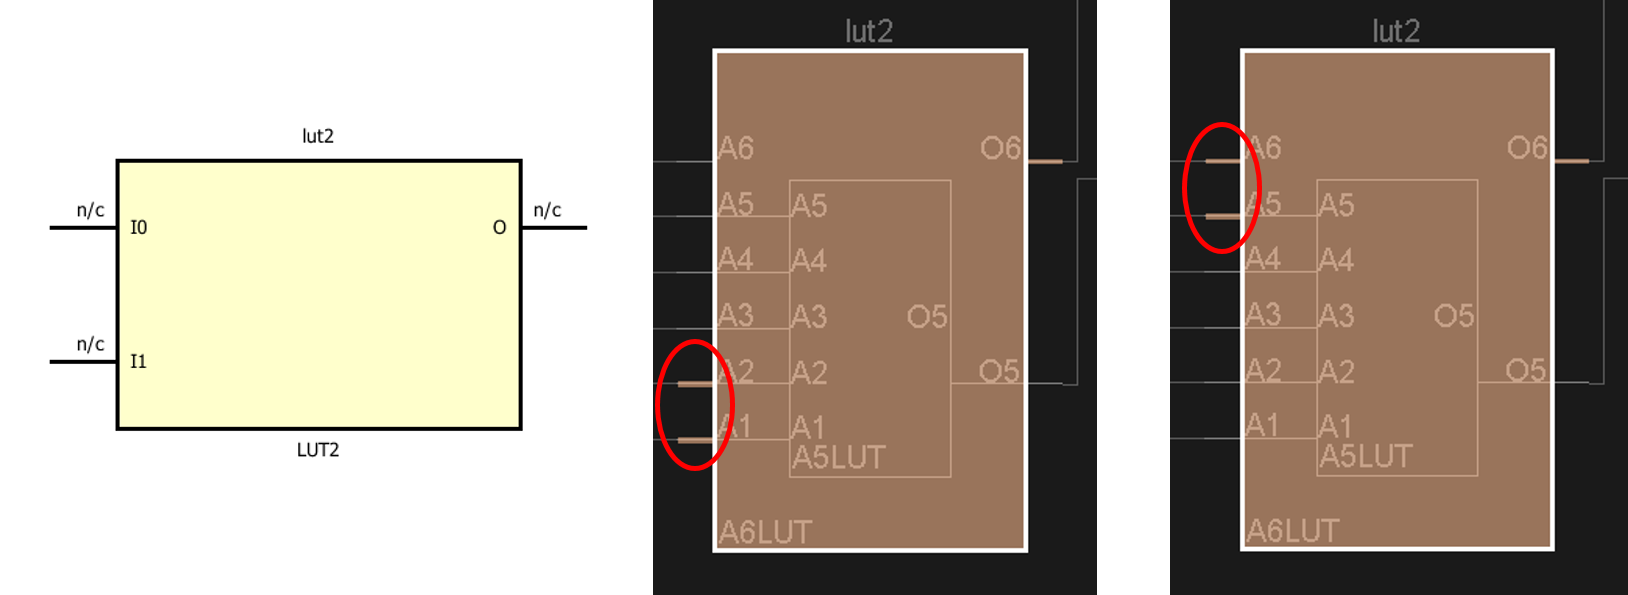
\includegraphics[width=1\columnwidth]{lutPins.png}
	\caption{LUT Pin Permutation Example}
	\label{fig:lutPins}
  \end{figure}
  
\vspace{.2cm}
\noindent
Some additional notes about placement are given in the list below: 

\begin {itemize}
  \item VCC and GND cells are not placed when implementing a design in Vivado.
  This distinction is applied to RapidSmith2 as well. Rather than placing VCC
  or GND explicitly, \texttt{RouteTree}s that are sourced by switchbox TIEOFFs
  are used to express their placement implicitly (VCC/GND is ``placed'' on the
  TIEOFF).
  
  \item A list of valid placement locations for a cell can be obtained with the
  function call \texttt{Cell::get\-Possible\-Anchors()}. The sample program
  \textbf{CreateDesignExample} demonstrates how to use this function.
 
  \item There are several placement rules for a given Xilinx FPGA. One such
  rule is that CARRY4 cells which are connected through a carry chain need
  to placed vertically to one another. Another example is that a RAMB36E1
  cell cannot be placed in the same tile as a RAMB18E1 cell. If either of these
  rules are violated, an error will be thrown in Vivado when attempting to
  import a design. It is the responsibility of the user to determine all
  relevant placement rules because error checking is not performed on design
  export.
  
  \item Macro cells in RapidSmith2 cannot be placed. The internal cells of a
  macro should be placed instead.
\end{itemize}
